\documentclass[10pt]{report}
\usepackage[utf8]{inputenc}
\usepackage[italian]{babel}
\usepackage{multicol}
\usepackage[a4paper, total={18cm, 25cm}]{geometry}
\usepackage{graphicx}
\graphicspath{ {./img/} }
\begin{document}
\title{Architettura degli Elaboratori}
\author{Appunti: Simone Pepi\\Stesura in \LaTeX: Federico Matteoni}
\date{ }
\renewcommand*\contentsname{Indice}

\maketitle
\tableofcontents
\pagebreak
\section{Introduzione}
Appunti del corso di \textbf{Architettura degli Elaboratori} presi a lezione da \textbf{Federico Matteoni}.\\\\
Prof.: \textbf{Maurizio Bonuccelli}, maurizio.angelo.bonuccelli@unipi.it\\
\begin{list}{-}{Riferimenti web:}
\item \emph{http://pages.di.unipi.it/bonuccelli/aeb.html}
\item \emph{didawiki.cli.di.unipi.it/doku.php/informatica/ae/start}
\end{list}
Ricevimento: Martedì 10-12, stanza 294 DE\\
Esame: \textbf{scritto} (\textit{closed book}) e \textbf{orale}. I compitini sono validi solo per la sessione invernale (gen-feb)\\
\begin{list}{-}{Libri}
\item  M. Vanneschi \textit{Architettura degli Elaboratori}, Pisa UniversitY Press
\item D. A. Patterson \textit{Computer Organization \& Design - The Hardware/Software Interface}
\end{list}
\section{Cosa riguarda il corso}
Consiste in come sono fatti pc internamento da un punto di vista di sottosistemi senza scendere nei dettagli elettrici.
\begin{list}{-}{Il corso è diviso in quattro parti:}
\item Fondamenti e strutturazione firmware (I Compitino)
\item Macchina assembler (D-RISC) e processi
\item Architetture General-Purpose
\item Architetture parallele (II Compitino)
\end{list}
\chapter{Fondamenti di strutturazione}
\section{Struttura a livelli}
\paragraph{Dividere} Per dedicarci allo studio di un sistema complesso spesso è utile \textbf{dividerlo in pezzi}. Nel caso di un sistema di elaborazione, in alcuni casi è \textbf{interessante avere una visione vicina alla struttura fisica} in termini di componenti hardware. In altri casi è \textbf{interessante avere una visione astratta del sistema} per poterne osservare le funzionalità e le strutture più adatte alla specifica applicazione.
\paragraph{Astrarre} Da questa necessità deriva la possibilità di strutturare un sistema a vari \textbf{livelli di astrazione} che non descrivono una reale struttura fisica, ma è \textbf{utile per ragioni specifiche} quali:
\begin{list}{}{}
\item Saper riconoscere \textbf{quale metodo di progettazione strutturata} viene seguito o conviene seguire (\textbf{top-down}, \textbf{bottom-up}, \textbf{middle-out})
\item Saper riconoscere \textbf{se i vari livelli rispettano una relazione gerarchica} oppure se non esiste alcun tipo di ordinamento
\item Essere in grado di \textbf{valutare a quali livelli conviene descrivere e implementare} determinate funzioni del sistema
\end{list}
\section{Macchine Virtuali}
\paragraph{Sistema di elaborazione} \textbf{Le funzionalità di un sistema di elaborazione} nel suo complesso possono essere \textbf{ripartite su un certo numero di livelli} che vengono definite \textbf{macchine virtuali}. \begin{list}{-}{La suddivisione può seguire \textbf{due approcci} fondamentali:}
	\item \textbf{Linguistico}: stabilisce i livelli in base ai linguaggi usati
	\item \textbf{Funzionale}: stabilisce i livelli in base a cosa fanno
\end{list}
I vari livelli sono schematizzati come in figura:
\begin{center}
\rule{5cm}{1pt} Interfaccia \rule{5cm}{1pt}\\
MV$_{i}$	R$_{i}$ = {risorse} + L$_{i}$ = {linguaggi}\\
\rule{5cm}{1pt} Interfaccia \rule{5cm}{1pt}\\
MV$_{i-1}$	R$_{i-1}$ = {risorse} + L$_{i-1}$ = {linguaggi}\\
\rule{5cm}{1pt} Interfaccia \rule{5cm}{1pt}\\
\end{center}
MV$_{i}$ realizza politica P$_{i}$ con linguaggio L$_{i}$ e risorse R$_{i}$.\\
MV$_{i}$ utilizza le funzionalità che il livello MV$_{i-1}$ (cioè le sue primitive) fornisce \textbf{attraverso l'interfaccia}.\\
L'interfaccia definita è fondamentale per poter rendere possibile la collaborazione tra le macchine virtuali, e permettere così ai linguaggi di MV$_{i}$ di sfruttare funzionalità e meccanismi di MV$_{i-1}$.\\
Le macchine virtuali godono delle \textbf{seguenti proprietà}:
\begin{list}{}{}
	\item L'\textbf{insieme} degli oggetti o risorse \textbf{R}$_{i}$ di MV$_{i}$ \textbf{è accessibile soltanto da parte dei meccanismi di L}$_{i}$ 
	\item Al livello MV$_{i}$ \textbf{non sono note le politiche adottate dai livelli inferiori}
\end{list}
\paragraph{Supporto a tempo di esecuzione} Anche detto \textbf{Runtime Support}, è l'\textbf{insieme dei livelli sottostanti}.\\
Nell'esempio, MV$_{i}$ ha come runtime support i livelli MV$_{i-1}$ \ldots MV$_{0}$.
\paragraph{Virtualizzazione ed Emulazione} Con \textbf{virtualizzazione} o astrazione intendiamo il \textbf{processo secondo cui un livello MV$_{i}$ usa funzionalità dei livelli superiori}.\\
Con \textbf{emulazione} o concretizzazione intendiamo il \textbf{processo secondo cui un livello MV$_{i}$ usa funzionalità dei livelli inferiori}.
\paragraph{Modularità} Tutte queste funzionalità sono \textbf{alla base della strutturazione di sistemi con elevata modularià}, \textbf{modificabilità}, \textbf{portabilità}, \textbf{manutebilità} e \textbf{testabilità}.
\subsection{Le Macchine Virtuali}
\begin{list}{}{}
\item \textbf{MV$_{4}$} Applicazioni\\L$_{4}$: Java, C, ML\ldots\\R$_{4}$: oggetti astratti, costrutti, tipi di dato definibili dall'utente
\item \rule{5cm}{1pt} \textit{Interfaccia}: chiamate di sistema \rule{5cm}{1pt}
\item \textbf{MV$_{3}$} Sistema Operativo\\L$_{3}$: C, linguaggi di programmazione concorrente, linguaggi sequenziali con librerie che implementano meccanismi di concorrenza\\R$_{3}$: variabili condivise, risorse condivise, oggetti astratti usati per la cooperazione tra processi e thread
\item \rule{5cm}{1pt} \textit{Interfaccia}: istruzioni assembler \rule{5cm}{1pt}
\item \textbf{MV$_{2}$} Macchina assembler\\L$_{2}$: assembler (D-RISC)\\R$_{2}$: registri, memoria, canali di comunicazione
\item \rule{5cm}{1pt} \textit{Interfaccia}: istruzioni firmware per l'assembler \rule{2.8cm}{1pt}
\item \textbf{MV$_{1}$} Firmware\\L$_{1}$: microlinguaggio\\R$_{1}$: sommatore, commutatore, registri, strutture di interconnessione intra-unità e inter-unità
\item \rule{5cm}{1pt} \textit{Interfaccia}: hardware \rule{6.7cm}{1pt}
\item \textbf{MV$_{0}$} Hardware\\L$_{0}$: \textit{funzionamento dei circuiti elettronici}\\R$_{0}$: circuiti elettronici elementari (AND, OR, NOT), collegamenti fisici, reti logiche
\end{list}
Il corso riguarderà principalmente i livelli MV$_{2}$ $\rightarrow$ MV$_{0}$ inclusi, comprese le istruzioni assembler.\\
Il livello firmware sarà fatto da \textbf{memoria}, \textbf{processore} e \textbf{dispositivi I/O}. I dispositivi di I/O comunicano bilateralmente con la memoria e il processore comunica bilateralmente con memoria. Opzionalmente, i dispositivi di I/O comunicano bilateralmente direttamente con il processore. Questa è l'\textbf{architettura standard}, presentata in maniera \textbf{estremamente semplicistica}.\\
Vedremo nel dettaglio il processore e la memoria, non i dispositivi di I/O perché troppo complessi.
\pagebreak
\subsection{Struttura Interna}
\paragraph{Da Verticale a Orizzontale} Fin'ora abbiamo parlato delle macchine virtuali in senso \textbf{verticale}, adesso vogliamo trovare un modo concettualmente uniforme -- \textbf{orizzontale} -- per poter studaire i livelli \textbf{al loro interno}.
\paragraph{Sistema di Elaborazione} Una volta scelta la struttura verticale di un sistema, dobbiamo capire come funziona l'interno di ciascun livello per poter far funzionare tutto il sistema, cioè dobbiamo capire \textbf{come funziona il sistema di elaborazione di un livello} composto da due componenti:
\begin{list}{}{}
	\item \textbf{Moduli di Elaborazione}, \textbf{ad ognuno} dei quali \textbf{è affidata l'elaborazione di un sottoinsieme di operazioni} del livello.
	\item \textbf{Struttura di Interconnessione}, \textbf{con la quale i moduli} di elaborazione del livello \textbf{cooperano e comunicano tra loro}.\\
	Essa può essere di due tipi:
\end{list}
\begin{center}
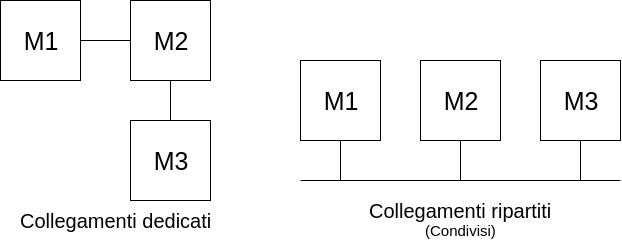
\includegraphics[scale=0.6]{strutturainterna.png}
\end{center}
\paragraph{Moduli di Elaborazione} Un modulo di elaborazione è definito come \textbf{un'entità autonoma e sequenziale}.
\subparagraph{Autonomia} L'autonomia è \textbf{data dal fatto che ogni modulo} di elaborazione \textbf{esegue un proprio controllo in maniera indipendente da altri moduli}.\\
Esso dunque \textbf{definisce le proprie strutture dati, operazioni elementari e interfacce} verso altri moduli.
\subparagraph{Sequenzialità} La sequenzialità è \textbf{data dal fatto che ogni modulo} di elaborazione \textbf{ha un singolo luogo di controllo}: \textbf{la sua attività è descritta} da un algoritmo di controllo costituito \textbf{da una lista sequenziale di comandi}.\\
La sequenzialità \textbf{non implica che un modulo non possa fare uso di forme di elaborazione concorrenti o parallele}. Alcuni o tutti i comandi di una lista sequenziale possono essere costituiti da una o più operazioni elementari \textbf{eseguite simultaneamente}.
\subsection{Parallelismo}
\paragraph{Sovrapporre} Poichè i moduli sono autonomi fra loro, sono in grado di \textbf{operare indipendentemente l'uno dall'altro}. \textbf{Le loro attività possono quindi essere sovrapposte nel tempo} eccetto quando, per ragioni legate alla sincronizzazione, alcuni di loro devono attendere il verificarsi di certi eventi dipendenti dall'elaborazione di altri.\\
In alcuni \textbf{casi limite} seppur realistici, il \textbf{funzionamento di tutti i moduli è rigidamente sequenziale}.\\\\
Tutto questo \textbf{vale per qualsiasi livello} o Macchina Virtuale, quindi sia per firmware che hardware.
\pagebreak
\subsection{Modelli di Cooperazione}
Dato un sistema di elaborazione a un certo livello, \textbf{i vari moduli} presenti \textbf{possono cooperare secondo due modalità}:
\begin{list}{}{}
	\item \textbf{Ambiente Globale}: esiste un \textbf{insieme di oggetti comuni accessibili da tutti i moduli} che devono cooperare tra loro, e \textbf{tutti i moduli possono operare su tale insieme}
	\item \textbf{Ambiente Locale}: \textbf{i moduli non condividono nulla}, quindi \textbf{non esiste alcun oggetto condivisio tra i moduli}. La \textbf{cooperazione avviene tramite scambio di messaggi}.
\end{list}
\begin{center}
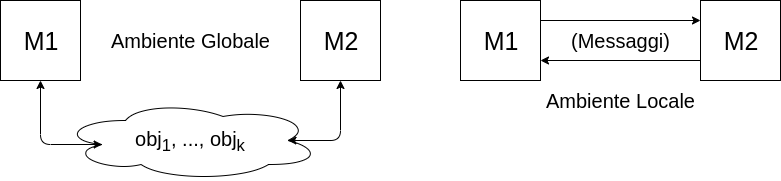
\includegraphics[scale=0.5]{modellicoop.png}
\end{center}
\pagebreak
\section{Compilazione vs Interpretazione}
\paragraph{Programmi} L'obiettivo di un calcolatore è \textbf{rendere possibile l'esecuzione di programmi} con una certa qualità di servizio. I programmi vengono \textbf{progettati mediante linguaggi di alto livello}, quindi \textbf{occorre operare una traduzione da linguaggio di alto livello a linguaggio assembler}.\\
Tale traduzione può essere effettuata tramite due ben note tecniche e loro combinazioni:
\begin{multicols}{2}
\textbf{Compilatore}: è \textbf{statico}.\\\textbf{Sostituisce l'intera sequenza del programma} sorgente con un sequenza di istruzioni assembler. Questa traduzione viene effettuata staticamente, vale a dire in fase di preparazione e \textbf{prima che il programma passi in esecuzione}.\\
Uno compilatore ha \textbf{completa visione del codice} e quindi \textbf{può ottimizzarlo}. La sua attività è analoga all'opera di un traduttore, che può leggersi il testo più volte per tradurlo alla perfezione.
\columnbreak

\textbf{Interprete}: è \textbf{dinamico}\\ Scandisce la sequenza \textbf{sostituendo ogni singolo comando} con una sequenza na di istruzioni assembler. La traduzione è effettuata dinamicamente, cioè \textbf{a tempo di esecuzione}, quindi non può ottimizzare. Il firmware riceve un'istruzione alla volta, quindi la interpreta.\\
Il suo svantaggio è che il \textbf{tempo di interpretazione viene pagato ogni volta che lancio il programma} e che \textbf{non può ottimizzare non avendo una visione globale} del programma.
\end{multicols}
Entrambe servono per tradurre il \textbf{codice sorgente} nel \textbf{programma oggetto} o \textbf{eseguibile}. L'esecuzione è quindi \textbf{più veloce in un programma compilato} rispetto ad un programma interpretato.
\begin{center}
\texttt{ADD R1, R2, R3} $\longrightarrow$ \textit{compilatore} $\longrightarrow$ \textbf{OBJ} $\longrightarrow$ Interprete Firmware (interfaccia tra MV ASM e MV FW)
\end{center}
Intuitivamente, dall'istruzione ad alto livello viene \textbf{compilato un programma oggetto OBJ} il quale è un insieme di bit che \textbf{viene interpretato dall'interprete firmware}.
\paragraph{Esempio} \textbf{Suppongo programmi}:\\
\begin{center}
	\begin{multicols}{2}
	\textbf{A}
	\begin{verbatim}
for i=0; i++; i<n
    A[i] = A[i] + B[i];
	\end{verbatim}

	\columnbreak
	\textbf{B}
	\begin{verbatim}
for i=0; i++; i<n
    B[i] = B[i] + C;
	\end{verbatim}
	\end{multicols}
\end{center}
Ricevendo i due blocchi di istruzioni, il \textbf{compilatore riconosce che sono diverse e le compila in modo diverso}. Però in entrambi i casi sono del tipo \textit{oggetto = somma due oggetti}, quindi produce una sequenza di istruzioni analoga (a meno di registri e dati, ovviamente).
Parte del secondo pezzo di codice, ad esempio, verrà tradotto in questa maniera:
\begin{multicols}{2}
\begin{list}{}{}
\item \texttt{LOAD R$_{base}$, R$_{I}$, R$_{1}$}
\item \texttt{ADD R$_{1}$, R$_{2}$, R$_{1}$}
\item \texttt{STORE R$_{base}$, R$_{I}$, R$_{1}$}
\item \texttt{INC R$_{I}$}
\item \texttt{IF$<$ R$_{I}$, R$_{N}$, LOOP}
\end{list}
\columnbreak
\begin{list}{}{}
\item \texttt{M[R[base] + R[I]] $\rightarrow$ R[1]}
\item \texttt{R[1] + R[2] $\rightarrow$ R[1]}
\item \texttt{R[1]  $\rightarrow$ M[R[base] + R[I]]}
\item \texttt{R[I] + 1 $\rightarrow$ R[I]}
\end{list}
\textbf{Microlinguaggio corrispondente}
\end{multicols}
\chapter{MV0 -- Hardware}
\section{Reti Logiche}
L'\textbf{implementazione a livello hardware di funzioni "pure"} dà luogo alle \textbf{Reti Combinatorie}.\\
L'\textbf{implementazione} a livello hardware \textbf{di funzioni "con stato"} dà luogo alle \textbf{Reti Sequenziali}.
\paragraph{Famiglia} Entrambe definiscono la famiglia delle \textbf{Reti Logiche} che permettono di \textbf{realizzare il livello hardware di un sistema di elaborazione}.
\section{Reti Combinatorie}
Una \textbf{rete combinatoria è} una rete logica \textbf{con \texttt{n} ingressi binari X$_{1}$ \ldots X$_{n}$ e \texttt{m} uscite binarie Z$_{1}$ \ldots Z$_{m}$}. Ad \textbf{ogni combinazione di valori in entrata corrisponde una ed una sola combinazione di valori in uscita}. La corrispondenza è definita secondo la funzione implementata dalla rete combinatoria.\\
Indichiamo X$_{1}$ \ldots X$_{n}$ e Z$_{1}$ \ldots Z$_{m}$ come \textbf{variabili logiche} di ingresso ed uscita. \textbf{Tutte le combinazioni possibili} delle variabili logiche \textbf{sono dette stati} di ingresso -- con 2$^n$ possibilità -- e di uscita -- 2$^m$ possibilità.\\\\
Pe rdescrivere le proprietà e la struttura interna delle reti combinatorie si usa un'\textbf{algebra isomorfa a quella logica}, chiama \textbf{Algebra Booleana}.
\subsection{Algebra Booleana}
L'algebra booleana è computata su \textbf{due valori} e \textbf{tre operatori}:
\begin{center}
\begin{multicols}{2}
\texttt{false}\\\texttt{true}\\
\columnbreak
\texttt{AND}\\\texttt{OR}\\\texttt{NOT}
\end{multicols}
\end{center}
Esistono anche altri operatori, derivati dai tre precedenti: \texttt{XOR}, \texttt{NAND}, \texttt{NOR} ecc..
\paragraph{Proprietà} Vale la proprietà distributiva anche per la somma rispetto alla moltiplicazione, oltre il viceversa, quindi: \texttt{A(B+C) = AB + AC}, ma anche \texttt{A + BC = (A + B)(A + C)}.\\
\begin{list}{-}{Inoltre si hanno le cosiddette \textbf{proprietà di DeMorgan}:}
\item \texttt{$\overline{A + B}$ = $\overline{A}$ * $\overline{B}$}
\item \texttt{$\overline{AB}$ = $\overline{A}$ + $\overline{B}$}
\end{list}
\begin{multicols}{3}
\subsubsection{AND}
Anche detta \textbf{moltiplicazione logica}.\\
\begin{tabular}{cc|c}
X & Y & Z \\
0 & 0 & 0 \\
0 & 1 & 0 \\
1 & 0 & 0 \\
1 & 1 & 1 \\
\end{tabular}
\columnbreak
\subsubsection{OR}
Anche detta \textbf{somma logica}.\\
\begin{tabular}{cc|c}
X & Y & Z \\
0 & 0 & 0 \\
0 & 1 & 1 \\
1 & 0 & 1 \\
1 & 1 & 1 \\
\end{tabular}
\columnbreak
\subsubsection{NOT}
Anche detta \textbf{negazione logica}.\\
\begin{tabular}{c|c}
Y & Z \\
0 & 1 \\
1 & 0 \\
\end{tabular}
\end{multicols}
Per costruire una \textbf{rete combinatoria} esistono varie tecniche. Quella che useremo si chiama \textbf{somma di prodotti}.
\subsection{Tecnica della Somma di Prodotti, o codifica degli 1}
\paragraph{La tecnica nel dettaglio} Partendo dalla \textbf{tabella di verità}, identifico le uscite che valgono 1. Di quelle uscite, \textbf{moltiplico (\texttt{AND})} tra loro le entrate \textbf{sulla stessa riga}, \textbf{nego le entrate che valgono 0} e \textbf{sommo (\texttt{OR}) tra loro le diverse righe}.
\paragraph{Un esempio con la somma algebrica} Partendo dalla seguente tabella di verità.\\
\begin{multicols}{2}
\begin{tabular}{cc|c|c}
X & Y & Z & R \\
0 & 0 & 0 & 0 \\
0 & 1 & 1 & 0 \\
1 & 0 & 1 & 0 \\
1 & 1 & 0 & 1\\
\end{tabular}
\columnbreak
\\Sfruttando la tecnica descritta sopra ottengo le seguenti espressioni per le due uscite:
\begin{list}{}{}
\item \texttt{Z = $\overline{X}$ * Y + X * $\overline{Y}$}
\item \texttt{R = X * Y}
\end{list}
\end{multicols}
Alternativamente, posso anche realizzare la \textbf{funzione complementare}, ovver fare il solito procedimento ma per le uscite che valgono 0 per poi negarle.\\
\begin{multicols}{2}
\begin{tabular}{cc|c|c}
X & Y & $\overline{Z}$ & R \\
0 & 0 & 1 & 0 \\
0 & 1 & 0 & 0 \\
1 & 0 & 0 & 0 \\
1 & 1 & 1 & 1\\
\end{tabular}
\columnbreak
\begin{list}{}{}
\item \texttt{Z = $\overline{\overline{X} * \overline{Y} + X * Y}$}
\item \texttt{R = X * Y}
\end{list}
\end{multicols}
\paragraph{Esempio}
\begin{center}
\begin{tabular}{cccc|c}
S1 & S2 & X & Y & S1* \\
0 & 0 & 0 & 0 & 0\\
0 & 0 & 0 & 1 & 0\\
0 & 0 & 1 & 0 & 0\\
0 & 0 & 1 & 1 & 1\\
0 & 1 & 0 & 0 & 0\\
0 & 1 & 0 & 1 & 0\\
0 & 1 & 1 & 0 & 0\\
0 & 1 & 1 & 1 & 1\\
1 & 0 & 0 & 0 & 0\\
1 & 0 & 0 & 1 & 1\\
1 & 0 & 1 & 0 & 1\\
1 & 0 & 1 & 1 & 1\\
1 & 1 & 0 & 0 & 0\\
1 & 1 & 0 & 1 & 1\\
1 & 1 & 1 & 0 & 1\\
1 & 1 & 1 & 1 & 1\\
\end{tabular}
\end{center}
S1* = $\overline{S1}$*$\overline{S2}$*X*Y + $\overline{S1}$*S2*X*Y + S1*$\overline{S2}$*$\overline{X}$*$\overline{Y}$ + S1*$\overline{S2}$*X*$\overline{Y}$ + S1*$\overline{S2}$*X*Y + S1*S2*$\overline{X}$*Y + S1*S2*X*$\overline{Y}$ + S1*S2*X*Y
\pagebreak
\subsection{Porte Logiche}
Una volta ricavata l'espressione logica dalla tabella di verità, è \textbf{immediato realizzare lo schema logico utilizzando le componenti hardware elementari}, dette anche \textbf{porte logiche}:
\begin{center}
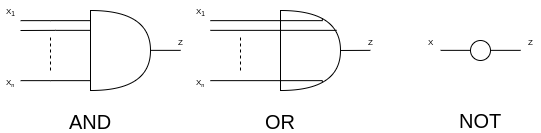
\includegraphics[scale=0.9]{portelogiche.png}
\end{center}
Ogni porta logica AND e OR \textbf{comporta un ritardo nel calcolo di 1 T$_p$}. Inoltre, ogni AND e OR può avere \textbf{massimo 8 ingressi}, quindi se ho più di 8 segnali in ingresso devo avere \textit{almeno} due livelli: un livello con tante porte logiche quando n/8 con n numero di segnali in ingresso, e \textit{almeno} un livello in cui "unire" i segnali in uscita in una porta logica analoga.
\subsection{Componenti Standard}
Di seguito sono le specifiche di alcune \textbf{reti combinatorie} che verranno supposte come \textbf{standard}, ovvero come componenti utilizzabili come blocchi elementari nella progettazione di strutture più complesse.
\subsubsection{Commutatore}
	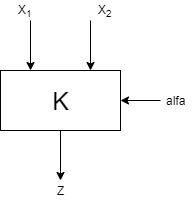
\includegraphics[scale=0.7]{commutatore.png}
\subsubsection{Selezionatore}
	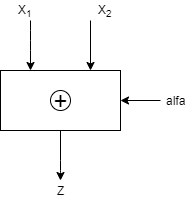
\includegraphics[scale=0.7]{confrontatore.png}
\subsubsection{Confrontatore}
	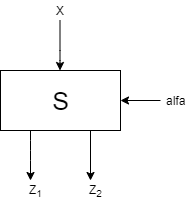
\includegraphics[scale=0.7]{selezionatore.png}
\subsubsection{ALU}
	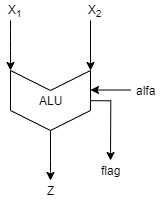
\includegraphics[scale=0.7]{ALU.png}
\subsection{Ritardo di Stabilizzazione}
\paragraph{Prestazioni} Per valutare le prestazioni di un sistema, occorre saper \textbf{valutare le prestazioni delle reti combinatorie}. Ogni rete reale è \textbf{caratterizzata da un ritardo T$_r$}, necessario affinché \textbf{a seguito di una variazione dello stato d'ingresso si produca la corrispondente variazione dello stato in uscita}.\\
\textbf{Solo dopo} questo tempo si dice che \textbf{la rete è stabilizzata}.
\paragraph{T$_p$} Per una porta logica indichiamo con T$_p$ \textbf{il ritardo di stabilizzazione} -- ad oggi è di circa 10$^{-2}$ millisecondi.\\
Supponiamo che le \textbf{porte NOT} abbiano un \textbf{ritardo nullo}, pari a 0 T$_p$, mentre per le \textbf{porte AND/OR} il valore T$_p$ dipende dal numero di ingressi n della porta. Per n $\leq$ 8 supponiamo che le porte AND/OR abbiano un \textbf{ritardo di stabilizzazione di 1 T$_p$}.\\
Il costo in T$_p$ sarà quindi pari ai livelli di AND/OR presenti. Ad esempio, se ho una tabella di verità con n termini ed m variabili, avrò log$_8$n livelli di OR e log$_8$m livelli di AND. Il costo in T$_p$ sarà quindi = (log$_8$n + log$_8$m) T$_p$
\subsection{Registri e memorie}
\pagebreak
\section{Reti Sequenziali}
Una \textbf{rete sequenziale} è un oggetto con \textbf{un ingresso ed una uscita}, capace di \textbf{mantenere uno stato interno} -- ecco perché si parla di funzioni con stato. A livello hardware, possiamo identificare una rete sequenziale con un \textbf{automa a stati finiti}.
\paragraph{ASF} Un \textbf{automa a stati finiti} è caratterizzato da:
\begin{list}{}{}
	\item n variabili di ingresso $\Rightarrow$ h = 2$^n$ \textbf{stati di ingresso} X$_1$\ldots X$_h$
	\item m variabili di uscita $\Rightarrow$ k = 2$^m$ \textbf{stati di uscita} Z$_1$\ldots Z$_k$
	\item r variabili logiche dello stato interno $\Rightarrow$ p = 2$^r$ \textbf{stati interni} S$_1$\ldots S$_p$
	\item una \textbf{funzione di transizione} dello stato interno $\sigma$: X x S $\rightarrow$ S che \textbf{definisce il passaggio tra gli stati}
	\item una \textbf{funzione delle uscite} $\omega$: X x S $\rightarrow$ Z che \textbf{calcola le uscite}
\end{list}
Una \textbf{rete sequenziale} è quindi \textbf{composta da due reti combinatorie $\sigma$ e $\omega$}, che rispettivamente calcolano la variazione dello stato e l'uscita, \textbf{e da un registro R} che contiene lo stato interno.
\subsection{Modello di Mealy}
\begin{multicols}{2}
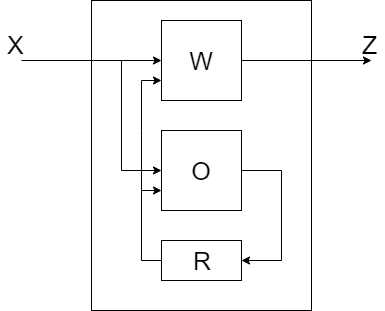
\includegraphics[scale=0.5]{mealy.png}
\columnbreak

Considerando il comportamento al tempo t, lo \textbf{stato interno successivo S(t+1)} dipende sia dallo stato di ingresso al tempo t, cioè X(t), sia dallo stato interno attuale S(t).\\
\texttt{S(t+1) = $\sigma$(X(t), S(t))}\\\\

Lo \textbf{stato di uscita al tempo t, Z(t)}, dipende sia dallo stato di ingresso X(t) sia dallo stato interno attuale S(t).\\
\texttt{Z(t) = $\omega$(X(t), S(t))}\\\\
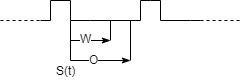
\includegraphics[scale=0.8]{clockmemo.png}
\end{multicols}
\subsection{Modello di Moore}
\begin{multicols}{2}
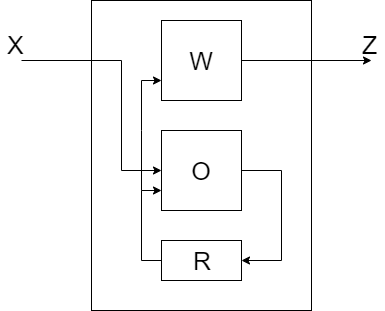
\includegraphics[scale=0.5]{moore.png}
\columnbreak

In maniera analoga al modello di Mealy, lo \textbf{stato interno successivo S(t+1)} dipende sia dallo stato di ingresso al tempo t, cioè X(t), sia dallo stato interno attuale S(t).\\
\texttt{S(t+1) = $\sigma$(X(t), S(t))}\\\\

Lo \textbf{stato di uscita al tempo t, Z(t)}, dipende solo dallo stato interno attuale S(t).\\
\texttt{Z(t) = $\omega$(S(t))}\\\\
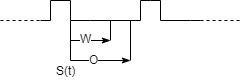
\includegraphics[scale=0.8]{clockmemo.png}
\end{multicols}
\pagebreak
\subsection{Reti Sequenziali di tipo Sincrono}
Vediamo adesso come si comportano nel tempo le reti sequenziali e spieghiamo perché adotteremo quelle di tipo sincrono. Come riferimento usiamo una rete di Mealy.
\paragraph{Spezzare} Abbiamo detto che lo stato al tempo successivo S(t + 1) dipende sia dall'ingresso X sia dallo stato interno attuale S(t), cioè \texttt{S(t+1) = $\sigma$(X(t), S(t))}.\\
Il registro R funge come un "cancello temporizzato" che \textbf{spezza la sequenza temporale degli eventi}.
\begin{multicols}{2}
Se il registro R non fosse presente, si verificherebbe la situazione in figura. In questo esempio, la porta logica o il componente $\sigma$ \textbf{potrebbero non stabilizzarsi mai}.\\
Se per esempio mettiamo una porta AND con due variabili in ingresso che nega il proprio risultato, tale rete tenderà a non stabilizzarsi mai ma a produrre una sequenza infinita di 0 e 1 in uscita.\\
Quindi devo avere necessariamente \textbf{un meccanismo che mi possa aiutare a determinare il valore dell'uscita} al tempo t, t + 1\ldots\\\\
Questo strumento è il resgistro impulsato, dove \textbf{la scrittura è scandita dal ciclo di clock}.
\columnbreak

\begin{center}
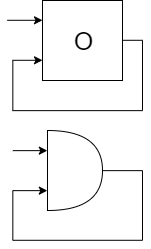
\includegraphics[scale=0.6]{esempiosincrono.png}
\end{center}
\end{multicols}
\paragraph{Modo Sincrono} Questo modo di lavorare delle reti sequenziali con un registro impulsato che funge da cancello temporizzato grazie al ciclo di clock si chiama \textbf{Modo Sincrono}.
\paragraph{Quando variare} Cerchiamo ora di capire quando devono variare gli ingressi e \textbf{per quanto tempo devono avere tale valore}.\\
Supponiamo di avere gli ingressi X$_0$ = 0 al tempo t, X$_1$ = 1 al tempo t + 1 e X$_2$ = 0 al tempo t + 2, e supponiamo che t$_\omega$ = t$_\sigma$ = 2t.
\begin{multicols}{2}
Se l'ingresso X variasse in un punto non precisato del ciclo di clock è probabile che $\omega$ e $\sigma$ non abbiano il \textbf{tempo necessario per produrre un risultato} e quindi avrei un \textbf{comportamento indefinito}.\\\\\\\\\\
In questo caso, cambiando il valore X all'inizio del ciclo di clock do il tempo necessario a $\sigma$ e $\omega$ di produrre un risultato stabile, ma al prossimo impulso del ciclo di clock (t + 2) leggerò di nuovo X = 1, che non è l'input corretto al tempo t + 2.\\\\\\\\\\\\
Questa è la soluzione giusta per il nostro esempio, che rispetta tutte le condizioni da noi elencate.
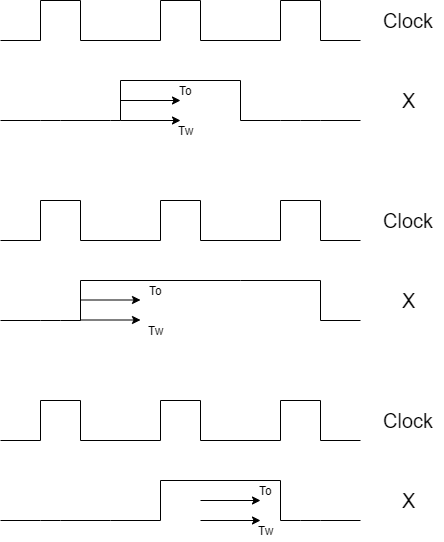
\includegraphics[scale=0.5]{sincronoesempi.png}
\end{multicols}
Per far funzionare le nostre reti, il ciclo di clock deve essere tale che T = MAX(t$_\sigma$, t$_\omega$) + $\delta$. Le reti funzionano anche con T $>$ MAX(t$_\sigma$, t$_\omega$) + $\delta$, ma avrei del \textbf{tempo perso} poiché la rete non opera, \textbf{aspetta solo che il clock sia alto per andare a scrivere nel registro}.
\pagebreak
\subsection{Reti Sequenziali a Componenti Standard}
Per poter sintetizzare una rete devo prima \textbf{decidere} se \textbf{implementare un modello di Mealy o di Moore}, \textbf{derivare le tabelle di verità} di $\omega$ e $\sigma$ e dire \textbf{quanti bit} ha il registro R.\\
Fatto questo, \textbf{ricavare le reti combinatorie} e \textbf{capire quanto valga il ciclo di clock} T (con T = MAX(t$_\sigma$, t$_\omega$) + $\delta$) che fa funzionare l'intera rete sequenziale.
\paragraph{Sintesi Classica} ASF $\longrightarrow$ Mealy o Moore $\rightarrow$ Tabelle verità, bit di R $\Rightarrow$ Reti combinatorie $\Rightarrow$ Ciclo di clock
\paragraph{Componenti Standard} In realtà per sintetizzare le reti sequenziali non usiamo questo procedimento di sintesi, ma bensì \textbf{usiamo i componenti standard}. Per esempio, prendiamo una rete che vuole calcolare il numero di persone presenti dentro una stanza con capienza massima 100 persone.
\paragraph{Con la sintesi classica} R ha bisogno di 7 bit per contare da 0 a 100.\\
Se andiamo, per esempio, a fare la tabella di verità per $\omega$, abbiamo ben 8 colonne negli ingressi, quindi 2$^8$ possibili combinazioni (righe).\\
Potrei avere 2$^8$/2 = 2$^7$ "uni" per colonna, di conseguenza un \textbf{numero considerevole di porte logiche}.\\
Diventa quindi praticamente impossibile sintetizzare questo esempio con il metodo classico. Procediamo con l'alternativa: l'utilizzo delle componenti standard.
\paragraph{Con le componenti standard} Procediamo col nostro esempio:\\
\begin{multicols}{2}
\begin{center}
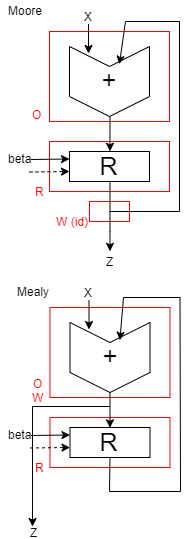
\includegraphics[scale=0.8]{esempiocompstd.png}
\end{center}
\columnbreak

In questo caso abbiamo usato il modello di Moore. Il \textbf{risultato è disponibile al prossimo impulso del ciclo di clock}.\\\\\\\\\\\\\\\\\\\\\\\\\\\\\\\\\\\\

Qua invece è stato usato il modello di Mealy. In questo caso si vede bene come \textbf{la rete di Mealy sia più veloce}, poiché \textbf{il risultato è subito disponibile} prima del prossimo impulso del ciclo di clock: infatti Z non viene scritto in R prima di essere pubblicato.
\end{multicols}
\pagebreak
Di seguito un esempio di rete sequenziale a componenti standard più complesso.
\begin{center}

\end{center}
\pagebreak
\section{Assembler D-RISC}
Istruzioni lunghe 32bit, primi 8bit per identificativo istruzione. Poi tre blocchi di 6Bit (R$_{i}$, R$_{j}$, R$_{h}$, in ogni blocco vi è mem semplicemente l'indice i, j o h). Poi 6 bit tipicamente inutilizzati (per estensioni future, istruzioni particolare e per riempire le locaz. di mem che sono tutte a 32 bit).\\
2$^{6}$ = 64 registri generali nel processore\\
Ad esempio \texttt{ADD R$_{i}$, R$_{j}$, R$_{h}$} significa \texttt{M[R[i] + R[j]] $\rightarrow$ R[h]}, e \texttt{ADD} è memorizzato con un determinato codice identificativo.\\
Per l'inizializzazione, ho il registro \texttt{R$_{0}$} che contiene sempre 0.

\paragraph{Esempio di RTS} \texttt{MV3 C = A + B}\\
Su MV$_{2}$ diventa \texttt{ADD R$_{A}$, R$_{B}$, R$_{C}$}\\
Su MV$_{1}$ ho registro A, registro B verso addizionatore/sottrattore (con alfa che indica operazione) e porta in C (con beta che indica scrittura attiva o meno)\\
Su MV$_{0}$ i vari componenti sono costruiti da una serie di gate (\texttt{AND}, \texttt{OR}, \texttt{NOT}).\\
\\
PO Parte Operativa\\
PC Parte Controllo\\
\texttt{roba eventuale}
\section{moduli operativi/unità funzionali}
Parte operativa: produce l'output\\
Parte controllo: dice alla PO \textit{come controllare} i suoi componenti (es. produe gli alfa (dicono cosa fare ai componenti) e i beta (quali registri in scrittura e quali no)). La PO porta alla PC le \textbf{variabili di condizionamento}, che istruiscono la PC su \textit{come} produrre alfa e beta.\\
PO e PC sono reti sequenziali.\\
In generale le mealY sono migliori: mediamente costano non di più e sono non più lente.\\
in mealY x va anche in omega.\\\\
1. PO --var condiz--> PC\\2. PC --alfa, beta-->PO\\3. PO --output Z--> \textit{fuori}\\
PO la faccio M-\\
PC la faccio M-\\
PO moore (ma non sarà automa), PC mealY\\\\
Funzionalmente MealY e Moore sono \textbf{equivalenti}. Moore rispodne dopo un clock, mealY risponde subito.\\
var condiz: info che PO passa alla PC affincché P generi alfa e beta.\\\\
microlinguaggio uao\\
\section{La Memoria}
\end{document}